El sonido es una perturbación mecánica que se propaga en medios elásticos ( aire, agua o sólidos ) y que percibimos a través del sistema auditivo.

Algunos conceptos importantes:

\begin{itemize}
    \item \textbf{1. Ondas Sonoras}

Las ondas sonoras son oscilaciones longitudinales que provocan variaciones en la presión del medio (ejemplo en Fig.1), zonas más densas (compresiones) y zonas menos densas (rarefacciones). Se generan por una fuente vibratoria, como una cuerda, un altavoz, cuerdas bucales o una gota de agua y esa vibración se transmite por colisión entre partículas del medio. \cite{sbe_sound}
\begin{figure}[H]
    \centering
    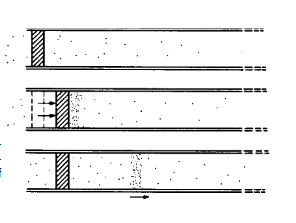
\includegraphics[width=0.7\textwidth]{commons/Fig1.png}
    \caption{Generación de una onda sonora longitudinal mediante el movimiento de un pistón al final de un tubo \cite{sbe_sound}.}
    \label{fig:ondas}
\end{figure}

    \item \textbf{2. Frecuencia y tono}

La frecuencia es el número de ciclos completos de la onda por segundo, medida en herzios (\textit{Hz}) y determina el tono de lo que escuchamos. Las notas tienen sus propias frecuencias, por ejemplo \textit{440Hz} corresponde a \textit{La4}, la voz humana suele ir en el rango 128-256 Hz , los ultrasonidos se consideran los superiores a 20 kHz y los infrasonidos los inferiores a 20 Hz \cite{libretexts_sound}. El rango de audición humana oscila entre los 20Hz y los 20kHz.

Por otro lado , el tono está relacionado con la \textit{frecuencia fundamental} ( aunque en sonidos complejos intervienen también armónicos, que son múltiplos de la frecuencia fundamental , lo cual afecta también al timbre , siendo el timbre lo que nos permite distinguir una misma nota tocada en una guitarra, un violín, o una flauta.)
    
    \item \textbf{3. Amplitud e intensidad}

La amplitud corresponde al máximo desplazamiento de las partículas en el medio respecto a su posición de equilibrio, reflejándose en el sonido como la magnitud de variación de presión o vibración.

Se percibe como \textit{volumen o sonoridad}, ondas con mayor amplitud suenan más fuertes.

La intensidad sonora mide la potencia transmitida por unidad de área (\textit{W/m²}) en la dirección del sonido y está relacionada con la amplitud al cuadrado\cite{openstax_intensity}:

\begin{center}
$I \propto A^2$
\end{center}

\end{itemize}